% Phase 1 final manuscript (IEEEtran, conference mode).
% Every number in this file is traceable to results/metrics/ or to the
% regenerated data artifacts; see reports/ieee_report/final_deliverables_verification.md.
% Compile:  pdflatex phase1_final_manuscript && bibtex phase1_final_manuscript
%           && pdflatex phase1_final_manuscript && pdflatex phase1_final_manuscript
\documentclass[conference]{IEEEtran}
\IEEEoverridecommandlockouts
\usepackage{cite}
\usepackage{amsmath,amssymb,amsfonts}
\usepackage{graphicx}
\usepackage{booktabs}
\usepackage{multirow}
\usepackage{xcolor}
\usepackage{url}
\usepackage[hidelinks]{hyperref}
\graphicspath{{figures/}}

\newcommand{\pmsem}[2]{#1\,$\pm$\,#2}

\begin{document}

\title{Molecular Toxicity Prediction Using Morgan Fingerprints and Physicochemical Descriptors: A Scaffold-Based Evaluation of Classical Machine Learning Models}

% Author names are taken from the repository README. Affiliations are placeholders
% to be completed by the authors; nothing here has been invented.
\author{
\IEEEauthorblockN{Amogha Raj Sindur, Bulbul Agarwalla, Shourya Pratap, Kanishka Dubey, Aditya Yadav}
\IEEEauthorblockA{\textit{[Department --- to be completed by authors]}\\
\textit{[Institution --- to be completed by authors]}\\
\textit{[City, Country]}\quad [contact e-mail]}
}

\maketitle

\begin{abstract}
In silico toxicity prediction can help prioritise compounds before costly experimental testing. However, public toxicity data are sparse and highly imbalanced, and reported accuracy depends strongly on how the data are split. We evaluate three classical classifiers (L2-regularised logistic regression, random forest and XGBoost) with three molecular representations: 2,048-bit Morgan fingerprints of radius~2, nine RDKit physicochemical descriptors, and their 2,057-dimensional concatenation. The task is the 12 nuclear-receptor and stress-response endpoints of the Tox21 dataset. After RDKit sanitisation, 7,823 of 7,831 records are retained. Data are partitioned with a deterministic Bemis--Murcko scaffold split (6,258/782/783 molecules) with no scaffold shared between partitions. Missing labels are masked rather than imputed, descriptor scaling is fitted on training data only, and decision thresholds are chosen on validation data only. On the held-out test partition, random forest with combined features obtains the highest macro ROC-AUC (0.7488) and macro average precision (0.3891) of the nine configurations. XGBoost with combined features is close behind on ROC-AUC (0.7456). For both tree ensembles, combining fingerprints with descriptors improved ROC-AUC over fingerprints alone on 11 of 12 endpoints. The across-endpoint standard errors (about 0.02) are comparable to the gaps between the leading models, and all results come from a single seed and a single split. Retraining in the pinned software environment reproduces the XGBoost results exactly but not the random-forest results (random forest with combined features scores 0.7625). We therefore report the comparison as descriptive rather than as evidence of a statistically established ranking.
\end{abstract}

\begin{IEEEkeywords}
Molecular toxicity prediction, Tox21, cheminformatics, Morgan fingerprints, molecular descriptors, scaffold splitting, random forest, imbalanced classification, reproducibility
\end{IEEEkeywords}

%=====================================================================
\section{Introduction}
%=====================================================================
Animal-based toxicity testing is slow and expensive, raises ethical concerns, and extrapolates imperfectly to humans~\cite{hartung2009toxicology}. The U.S. National Research Council therefore proposed moving toxicity assessment toward high-throughput \textit{in vitro} assays of toxicity pathways~\cite{nrc2007toxicity}. The Tox21 programme put this into practice: it screened a library of roughly 10,000 environmental chemicals and drugs, and the 2014 Tox21 Data Challenge released 12 nuclear-receptor (NR) and stress-response (SR) assays as a public modelling benchmark~\cite{huang2016tox21}. Computational models trained on such data can be used to prioritise compounds for experimental follow-up.

Three properties of Tox21 make honest evaluation difficult. First, the compound--assay label matrix is incomplete, because not every compound was tested in every assay. Second, active compounds are rare. Third, molecules cluster into structurally related series. Under a random split, close analogues of a test compound are likely to appear in the training set, which can make performance estimates optimistic. Scaffold-based splitting separates molecules by their Bemis--Murcko framework~\cite{bemis1996frameworks} and is described by MoleculeNet as a more challenging protocol than random splitting~\cite{wu2018moleculenet}. Notably, MoleculeNet itself benchmarks Tox21 with a \emph{random} split~\cite{wu2018moleculenet}.

Classical learners with handcrafted representations remain strong baselines. Random forests~\cite{breiman2001random} were established as accurate QSAR models by Svetnik \textit{et al.}~\cite{svetnik2003random}. Gradient boosting has performed comparably to random forests on cheminformatics data~\cite{svetnik2005boosting}. In a comparison across 11 public datasets, Jiang \textit{et al.} found that descriptor-based models on average outperformed graph neural networks~\cite{jiang2021could}. A rigorous classical baseline is therefore a necessary reference point before learned graph representations are considered.

This paper reports Phase~1 of a two-phase project. The question is: \emph{under a leakage-controlled scaffold split of Tox21, how do circular fingerprints, physicochemical descriptors and their combination compare when used with logistic regression, random forest and XGBoost?} The contributions are:
\begin{enumerate}
\item A reproducible, checksum-verified Tox21 curation and Bemis--Murcko scaffold-split pipeline with no scaffold overlap between partitions.
\item A $3\times3$ benchmark (models $\times$ representations) over 12 endpoints. Missing labels are masked, descriptor scaling uses training data only, and decision thresholds use validation data only.
\item Endpoint-level analysis relating ranking performance (ROC-AUC) and precision-oriented performance (average precision) to class prevalence.
\item A transparent uncertainty and reproducibility analysis. We state what the reported spread does and does not measure, and we report the result of retraining in the pinned environment.
\end{enumerate}
Graph neural networks are \emph{not} evaluated here and are discussed only as future work.

%=====================================================================
\section{Related Work}
%=====================================================================
\subsection{Tox21 and Computational Toxicology}
The Tox21 Data Challenge evaluated models on 12 assays, with AUC-ROC as the primary metric, on a 641-compound evaluation set assembled specifically for the challenge~\cite{huang2016tox21}. The winning models reached ROC-AUC values between 0.81 and 0.95 across sub-challenges. The androgen-receptor assays were among the hardest, at about 0.7~\cite{huang2016tox21}. The overall winner, DeepTox, combined multi-task deep networks with large sets of descriptors, toxicophores and fingerprints~\cite{mayr2016deeptox}. In its published comparison, random forests and SVMs trailed the deep network by small average margins~\cite{mayr2016deeptox}. These results use the challenge's own test set rather than a scaffold split, so they are context and not a target for direct numerical comparison.

\subsection{Molecular Representations}
Descriptor-based QSAR dates back to the linear free-energy models of Hansch and Fujita~\cite{hansch1964rho}; Todeschini and Consonni catalogue thousands of descriptors~\cite{todeschini2009descriptors}. The descriptors used here have well-documented origins. The atom-contribution $\log P$ comes from Wildman and Crippen~\cite{wildman1999logp}, the fragment-based topological polar surface area from Ertl \textit{et al.}~\cite{ertl2000tpsa}, hydrogen-bond donor and acceptor counts from Lipinski \textit{et al.}~\cite{lipinski1997rule}, and the fraction of $sp^3$ carbons from Lovering \textit{et al.}~\cite{lovering2009flatland}. Such global properties summarise size, polarity and lipophilicity but lose substructural detail. Extended-connectivity fingerprints (ECFP)~\cite{rogers2010ecfp}, which build on the Morgan algorithm~\cite{morgan1965generation}, encode circular atom neighbourhoods as hashed bits. They capture local functional groups at the cost of hash collisions and a representation that cannot adapt to the task. The two families are complementary in principle, which motivates testing their concatenation.

\subsection{Classical Learners for Molecular Classification}
Random forests aggregate decorrelated trees grown on bootstrap samples~\cite{breiman2001random}. They are robust and accurate in QSAR settings~\cite{svetnik2003random}. Stochastic gradient boosting has been reported to perform comparably to random forests on ten cheminformatics datasets~\cite{svetnik2005boosting}. XGBoost adds second-order optimisation and regularisation of tree complexity~\cite{chen2016xgboost}. Jiang \textit{et al.} report that random forests and XGBoost give reliable classification performance at low computational cost~\cite{jiang2021could}. Yang \textit{et al.} likewise benchmark fingerprint and descriptor models against learned graph representations to test generalisation to new chemical space~\cite{yang2019analyzing}. Our study does not propose a new learner. Its contribution is a controlled comparison of representations under one leakage-aware protocol.

\subsection{Splitting, Leakage and Evaluation}
Random cross-validation can overestimate prospective QSAR performance, as Sheridan showed by contrasting random selection with time-split validation~\cite{sheridan2013time}. Scaffold splitting~\cite{bemis1996frameworks,wu2018moleculenet} is a structure-based alternative for datasets without timestamps, such as Tox21. More broadly, Kapoor and Narayanan document data leakage as a widespread cause of irreproducible, over-optimistic results in ML-based science~\cite{kapoor2023leakage}. That finding motivates our training-only preprocessing and validation-only threshold selection. For imbalanced data, the precision--recall view is more informative than ROC~\cite{saito2015precision}, and Davis and Goadrich formalise the relationship between the two curves~\cite{davis2006relationship}. We therefore report average precision alongside ROC-AUC.

%=====================================================================
\section{Dataset and Problem Formulation}
%=====================================================================
\subsection{Source and Curation}
The dataset is the DeepChem distribution of Tox21 (\texttt{tox21.csv.gz}, 122,925 bytes). Its SHA-256 checksum (\texttt{45d09792\ldots0c0d360}) is verified on every download. The file contains 7,831 records, each with a SMILES string, a molecule identifier and 12 endpoint columns. Each SMILES is parsed and sanitised with RDKit~\cite{rdkit} and converted to canonical isomeric SMILES. Eight records fail sanitisation because aluminium atoms exceed RDKit's permitted explicit valence. These records are excluded and logged rather than repaired, which leaves 7,823 molecules with distinct canonical SMILES (no duplicate groups). The exclusion reflects this pipeline's sanitisation criteria; it does not imply the structures are chemically meaningless.

\subsection{Labels}
Each endpoint label $y_{ik}\in\{0,1,\varnothing\}$ marks molecule $i$ as inactive, active or untested on assay $k$. Of the $7{,}823\times12=93{,}876$ molecule--endpoint pairs, 77,864 are labelled and 16,012 (17.06\%) are missing. Positive prevalence among labelled pairs ranges from 2.89\% (NR-PPAR-gamma) to 16.17\% (SR-ARE) (Table~\ref{tab:labels}, Fig.~\ref{fig:labels}). Missing labels are never treated as negatives. Each endpoint is modelled as a separate binary task trained on its labelled molecules only.

\begin{table}[t]
\caption{Label statistics of the 7,823 curated molecules}
\label{tab:labels}
\centering
\footnotesize
\setlength{\tabcolsep}{4pt}
\begin{tabular}{lrrrr}
\toprule
Endpoint & Active & Inactive & Missing (\%) & Prev. (\%)\\
\midrule
NR-AR          & 308 & 6,950 & 7.22  & 4.24\\
NR-AR-LBD      & 237 & 6,514 & 13.70 & 3.51\\
NR-AhR         & 768 & 5,774 & 16.37 & 11.74\\
NR-Aromatase   & 300 & 5,515 & 25.67 & 5.16\\
NR-ER          & 791 & 5,395 & 20.93 & 12.79\\
NR-ER-LBD      & 349 & 6,599 & 11.18 & 5.02\\
NR-PPAR-gamma  & 186 & 6,257 & 17.64 & 2.89\\
SR-ARE         & 942 & 4,883 & 25.54 & 16.17\\
SR-ATAD5       & 264 & 6,801 & 9.69  & 3.74\\
SR-HSE         & 372 & 6,088 & 17.42 & 5.76\\
SR-MMP         & 918 & 4,886 & 25.81 & 15.82\\
SR-p53         & 423 & 6,344 & 13.50 & 6.25\\
\bottomrule
\end{tabular}
\end{table}

\begin{figure}[t]
\centering
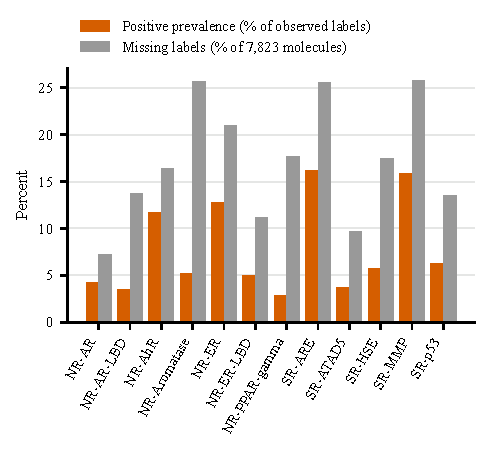
\includegraphics[width=\columnwidth]{fig_label_statistics}
\caption{Per-endpoint positive prevalence (percent of labelled molecules) and label missingness (percent of all 7,823 molecules).}
\label{fig:labels}
\end{figure}

%=====================================================================
\section{Molecular Representations}
%=====================================================================
\textbf{Morgan fingerprints.} For each molecule, RDKit's \texttt{GetMorganGenerator} with radius $r=2$ (ECFP4-like) and default atom invariants produces a binary vector $\mathbf{x}^{\mathrm{M}}\in\{0,1\}^{2048}$. Each circular environment identifier $s$ sets bit $h(s)\bmod 2048$, where $h$ is RDKit's hash. Stereochemistry is not included (the RDKit default).

\textbf{Descriptors.} The vector $\mathbf{x}^{\mathrm{D}}\in\mathbb{R}^{9}$ contains average molecular weight, Wildman--Crippen $\log P$~\cite{wildman1999logp}, TPSA~\cite{ertl2000tpsa}, H-bond donors and acceptors~\cite{lipinski1997rule}, rotatable bonds, ring count, heavy-atom count and fraction of $sp^3$ carbons~\cite{lovering2009flatland}, all computed with RDKit.

\textbf{Combined.} The vector $\mathbf{x}^{\mathrm{C}}=[\mathbf{x}^{\mathrm{M}}\,\|\,\mathbf{x}^{\mathrm{D}}]\in\mathbb{R}^{2057}$ is the concatenation of the two.

\textbf{Leakage-safe scaling.} Descriptors are standardised as $z_j=(x_j-\mu_j^{\mathrm{tr}})/(\sigma_j^{\mathrm{tr}}+\epsilon)$, where $\mu_j^{\mathrm{tr}}$ and $\sigma_j^{\mathrm{tr}}$ are estimated on training molecules only and $\epsilon=10^{-8}$. Morgan bits are left unscaled. No feature uses label information.

%=====================================================================
\section{Experimental Methodology}
%=====================================================================
Fig.~\ref{fig:pipeline} summarises the pipeline.

\begin{figure*}[t]
\centering
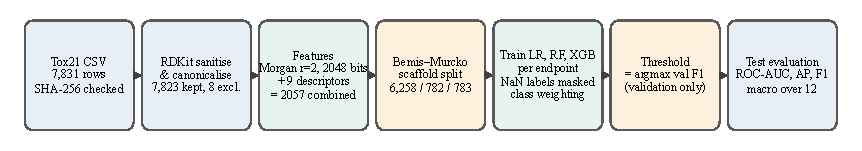
\includegraphics[width=\textwidth]{fig_pipeline}
\caption{Phase~1 pipeline. Test labels are used only in the final evaluation step.}
\label{fig:pipeline}
\end{figure*}

\subsection{Scaffold Split}
Each molecule's Bemis--Murcko scaffold~\cite{bemis1996frameworks} is computed with RDKit (\texttt{MurckoScaffoldSmiles}, chirality excluded). Molecules are grouped by scaffold. The 1,775 acyclic molecules, whose scaffold is empty, form a single group. Groups are sorted by size in descending order, ties are shuffled with seed~42, and groups are assigned greedily: to the training partition until it reaches 80\% of molecules, then to validation until 10\%, and the remainder to test. The result is 6,258 / 782 / 783 molecules with 760 / 782 / 783 distinct scaffolds. Independent re-extraction of scaffolds confirmed zero overlap between partitions. Because the largest groups are assigned first, the validation and test partitions consist entirely of singleton scaffolds. They therefore measure generalisation to rare, structurally isolated chemotypes, which is one form of out-of-distribution evaluation among several.

\subsection{Models and Training}
For each representation and each endpoint $k$, an independent binary classifier is trained on the training molecules labelled for $k$. Hyperparameters were fixed in advance and not tuned (Table~\ref{tab:hparams}). Models are implemented with scikit-learn~\cite{pedregosa2011scikit} and XGBoost~\cite{chen2016xgboost}. Class imbalance is handled by inverse-frequency class weights for LR and RF and by $\texttt{scale\_pos\_weight}=N^{-}_{k}/N^{+}_{k}$ (training counts) for XGBoost. All models use \texttt{random\_state}~=~42.

\begin{table}[t]
\caption{Fixed hyperparameters (no tuning was performed)}
\label{tab:hparams}
\centering
\footnotesize
\begin{tabular}{ll}
\toprule
Model & Configuration\\
\midrule
LR      & L2, $C=1.0$, lbfgs, max\_iter 1000, balanced weights\\
RF      & 100 trees, max\_depth 12, min\_samples\_split 5, balanced\\
XGBoost & 100 rounds, max\_depth 5, $\eta=0.1$, scale\_pos\_weight\\
\bottomrule
\end{tabular}
\end{table}

\subsection{Threshold Selection and Test Isolation}
The validation partition is used for exactly one purpose: choosing, for each endpoint, the decision threshold
\begin{equation}
\tau_k^{*}=\arg\max_{\tau\in\{0.05,0.06,\ldots,0.95\}} F_1\!\left(\mathbf{y}^{\mathrm{val}}_{k},\,\mathbb{1}[\hat{\mathbf{p}}^{\mathrm{val}}_{k}\ge\tau]\right),
\end{equation}
which is then applied unchanged to the test partition. Test labels are not used for training, scaling, threshold selection or model choice. A regression test verifies that the selected threshold is unaffected by test labels.

%=====================================================================
\section{Evaluation Metrics}
%=====================================================================
For endpoint $k$, all metrics are computed on the labelled subset $\mathcal{S}_k=\{i: y_{ik}\neq\varnothing\}$ of the test partition. \textbf{ROC-AUC} is the probability that a random active compound is scored above a random inactive one. \textbf{Average precision} (AP), reported as ``PR-AUC'', is
\begin{equation}
\mathrm{AP}_k=\sum_{n}(R_n-R_{n-1})P_n,
\end{equation}
where $P_n$ and $R_n$ are precision and recall at the $n$-th score threshold. This is the step-wise estimator, not the trapezoidal area. A random ranker's AP equals the endpoint's prevalence, so AP must be read relative to that baseline. \textbf{F$_1$} and \textbf{balanced accuracy} are computed at $\tau_k^{*}$. If an endpoint had only one class in a partition, its ranking metrics would be undefined (NaN) and excluded from the average. This did not occur in the present split.

\textbf{Aggregation and uncertainty.} For a metric $M$ with endpoint values $M_1,\ldots,M_K$ ($K=12$),
\begin{equation}
\bar M=\frac1K\sum_{k}M_k,\quad s=\sqrt{\tfrac{1}{K-1}\sum_k(M_k-\bar M)^2},\quad \mathrm{SEM}=\frac{s}{\sqrt K}.
\end{equation}
The reported ``$\pm$'' is this SEM \emph{across endpoints within a single run}. It summarises how much performance varies across assays. It is \emph{not} an estimate of run-to-run, seed or resampling variability, and it is not a significance test between models.

%=====================================================================
\section{Results}
%=====================================================================
\subsection{Benchmark}
Table~\ref{tab:main} and Fig.~\ref{fig:compare} report test-partition results for all nine configurations. These values are recomputed exactly (to four decimals) from the saved per-molecule prediction files using an independent scikit-learn implementation.

\begin{table*}[t]
\caption{Test-partition results (783 molecules, 12 endpoints). ``$\pm$'' is the SEM across endpoints from one run (seed 42); SD is the across-endpoint standard deviation. F$_1$ and balanced accuracy (BA) are at validation-selected thresholds. Best value per column in bold.}
\label{tab:main}
\centering
\footnotesize
\begin{tabular}{llr cc cc cc}
\toprule
Model & Representation & Dim. & ROC-AUC (mean $\pm$ SEM) & ROC-AUC SD & AP (mean $\pm$ SEM) & AP SD & Macro F$_1$ & Macro BA\\
\midrule
\multirow{3}{*}{LR} & Morgan      & 2048 & \pmsem{0.6987}{0.0149} & 0.0515 & \pmsem{0.2602}{0.0341} & 0.1182 & 0.3001 & 0.6216\\
                    & Descriptors & 9    & \pmsem{0.7203}{0.0169} & 0.0585 & \pmsem{0.1968}{0.0397} & 0.1376 & 0.2472 & 0.6188\\
                    & Combined    & 2057 & \pmsem{0.7138}{0.0158} & 0.0546 & \pmsem{0.2341}{0.0338} & 0.1172 & 0.3159 & 0.6404\\
\midrule
\multirow{3}{*}{RF} & Morgan      & 2048 & \pmsem{0.7208}{0.0199} & 0.0688 & \pmsem{0.3458}{0.0316} & 0.1095 & 0.3712 & 0.6475\\
                    & Descriptors & 9    & \pmsem{0.7215}{0.0216} & 0.0747 & \pmsem{0.2901}{0.0408} & 0.1413 & 0.3036 & 0.6337\\
                    & Combined    & 2057 & \textbf{\pmsem{0.7488}{0.0181}} & 0.0628 & \textbf{\pmsem{0.3891}{0.0320}} & 0.1108 & \textbf{0.3781} & \textbf{0.6636}\\
\midrule
\multirow{3}{*}{XGBoost} & Morgan      & 2048 & \pmsem{0.7114}{0.0181} & 0.0627 & \pmsem{0.3027}{0.0308} & 0.1067 & 0.3351 & 0.6340\\
                         & Descriptors & 9    & \pmsem{0.7024}{0.0256} & 0.0887 & \pmsem{0.2911}{0.0454} & 0.1574 & 0.3133 & 0.6394\\
                         & Combined    & 2057 & \pmsem{0.7456}{0.0179} & 0.0620 & \pmsem{0.3495}{0.0406} & 0.1407 & 0.3591 & 0.6485\\
\bottomrule
\end{tabular}
\end{table*}

\begin{figure*}[t]
\centering
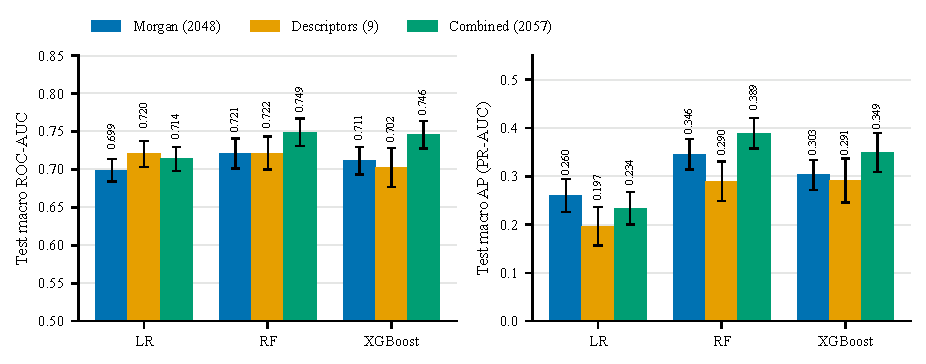
\includegraphics[width=\textwidth]{fig_model_comparison}
\caption{Test macro ROC-AUC (left) and AP (right) for each model and representation. Error bars show the SEM across the 12 endpoints (single run), not run-to-run uncertainty.}
\label{fig:compare}
\end{figure*}

RF with combined features obtains the highest value on every macro metric. XGBoost with combined features is close on ROC-AUC (0.7456 against 0.7488). At the endpoint level the two are effectively tied on ROC-AUC, with RF ahead on 6 of 12 endpoints and a median paired difference of 0.001. RF is ahead on AP for 8 of 12 endpoints. Both differences are small relative to the across-endpoint SEM of about 0.02.

Combining the two representations helps both tree ensembles consistently. Relative to Morgan alone, combined features raise ROC-AUC on 11 of 12 endpoints for both RF and XGBoost, and raise AP on 11 (RF) and 10 (XGBoost) endpoints. Relative to descriptors alone, combined features raise ROC-AUC on 9 (RF) and 8 (XGBoost) endpoints. Logistic regression behaves differently. Its best ROC-AUC comes from the nine descriptors (0.7203), but this configuration has the lowest AP of all nine (0.1968). Adding descriptors to fingerprints raised LR's AP on only 3 of 12 endpoints.

\subsection{Endpoint-Level Behaviour}
Table~\ref{tab:endpoints} and Fig.~\ref{fig:endpoints} break down the leading configuration by endpoint. Test ROC-AUC ranges from 0.662 (SR-ARE) to 0.852 (NR-AhR). AP exceeds the prevalence baseline on every endpoint, from 1.7$\times$ the baseline (SR-ARE) to 19$\times$ (NR-AR-LBD). The two metrics rank endpoints differently. NR-AR-LBD has high ROC-AUC (0.818) but only 14 active test compounds, while NR-AR has low ROC-AUC (0.670) yet high precision (0.875) and low recall (0.280) at its threshold. Across the 12 endpoints, test prevalence correlates more strongly with AP (Pearson $r=0.52$) and F$_1$ ($r=0.61$) than with ROC-AUC ($r=0.22$). This is consistent with AP and F$_1$ depending on class balance.

\begin{table}[t]
\caption{Test results per endpoint for RF with combined features. $\tau^*$: validation-selected threshold; Pos./Obs.: active compounds over labelled compounds in the test partition}
\label{tab:endpoints}
\centering
\footnotesize
\setlength{\tabcolsep}{3.2pt}
\begin{tabular}{lcccccr}
\toprule
Endpoint & $\tau^*$ & ROC-AUC & AP & Prev. & F$_1$ & Pos./Obs.\\
\midrule
NR-AR         & 0.69 & 0.670 & 0.335 & 0.035 & 0.424 & 25/722\\
NR-AR-LBD     & 0.40 & 0.818 & 0.421 & 0.022 & 0.323 & 14/631\\
NR-AhR        & 0.54 & 0.852 & 0.539 & 0.146 & 0.480 & 92/632\\
NR-Aromatase  & 0.55 & 0.758 & 0.304 & 0.079 & 0.300 & 41/517\\
NR-ER         & 0.54 & 0.726 & 0.428 & 0.122 & 0.391 & 69/566\\
NR-ER-LBD     & 0.54 & 0.730 & 0.486 & 0.041 & 0.476 & 27/663\\
NR-PPAR-gamma & 0.38 & 0.707 & 0.201 & 0.048 & 0.178 & 28/579\\
SR-ARE        & 0.50 & 0.662 & 0.365 & 0.210 & 0.415 & 99/472\\
SR-ATAD5      & 0.45 & 0.715 & 0.295 & 0.038 & 0.216 & 25/663\\
SR-HSE        & 0.47 & 0.774 & 0.367 & 0.078 & 0.393 & 44/561\\
SR-MMP        & 0.51 & 0.846 & 0.594 & 0.216 & 0.611 & 114/527\\
SR-p53        & 0.52 & 0.729 & 0.335 & 0.097 & 0.331 & 62/642\\
\bottomrule
\end{tabular}
\end{table}

\begin{figure}[t]
\centering
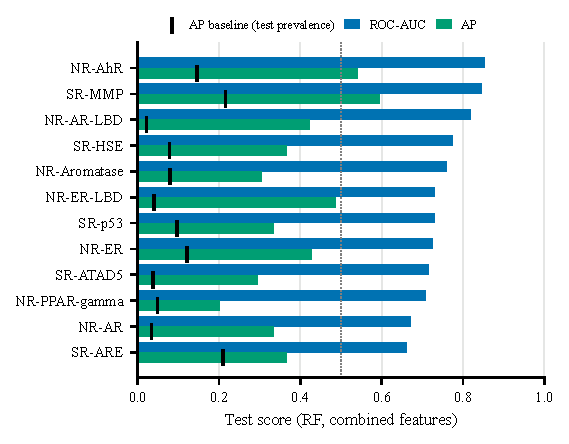
\includegraphics[width=\columnwidth]{fig_endpoint_rf_combined}
\caption{Per-endpoint test ROC-AUC and AP for RF with combined features, sorted by ROC-AUC. Black ticks mark each endpoint's test prevalence, the expected AP of a random ranker.}
\label{fig:endpoints}
\end{figure}

\subsection{Reproducibility Check}\label{sec:repro}
All pipeline stages were regenerated from the raw download in the pinned environment (Python~3.12, scikit-learn~1.9.1, XGBoost~3.4.1, RDKit~2026.9.1). The data, features and split matched the documented values, and the project's 122 automated tests passed. Retraining reproduced the XGBoost predictions and LR with descriptors byte-for-byte. It did \emph{not} reproduce RF: RF with combined features scored \pmsem{0.7625}{0.0196} ROC-AUC and 0.4046 AP, compared with the 0.7488 and 0.3891 committed. LR with Morgan or combined features shifted by at most 0.0002 in ROC-AUC. Retraining was deterministic within the environment, and the evaluation code is unchanged since the results were committed. The reported results were produced before library versions were pinned, so the most likely cause is a difference in the scikit-learn version. The ranking of configurations was unchanged. We report the committed values because they are the archived predictions that every other project artifact refers to.

%=====================================================================
\section{Discussion}
%=====================================================================
\textbf{Why combine representations?} Morgan bits record which local substructures are present. The descriptors summarise global size, polarity and lipophilicity, which no single bit encodes. Tree ensembles can use both kinds of signal, and the improvements on 10--11 of 12 endpoints suggest that they do. This study does not establish a mechanism, and we do not attribute the gain to specific descriptors. With LR, the nine scaled descriptors sit alongside 2,048 sparse binary columns under a single L2 penalty, which may explain why concatenation helped LR's AP so rarely.

\textbf{Ranking versus thresholded metrics.} ROC-AUC treats all thresholds as equally relevant and does not depend on prevalence. AP and F$_1$ reflect how many retrieved compounds are truly active, which matters when only a few top-ranked compounds can be tested experimentally~\cite{saito2015precision}. On SR-ARE, for example, ROC-AUC is the lowest (0.662) but AP (0.365) is mid-range, because its test prevalence is the highest (21\%). Reporting only ROC-AUC would hide this.

\textbf{Effect of the split.} The test partition contains only singleton scaffolds, and its class balance differs from the full dataset: SR-ARE has 16.2\% actives overall but 21.0\% in test, and NR-AR-LBD has 3.5\% overall but 2.2\% in test. Endpoint results therefore depend on a small number of actives, as few as 14. Our numbers are not comparable to MoleculeNet's random-split Tox21 results~\cite{wu2018moleculenet} or to the Tox21 Challenge leaderboard~\cite{huang2016tox21}, which used a different test set. With that caveat, the androgen-receptor assay (NR-AR) was also among the hardest endpoints in the challenge~\cite{huang2016tox21}.

\textbf{How to read the ranking.} RF with combined features is the best of the nine configurations \emph{under this protocol}. Its margin over XGBoost with combined features is within the across-endpoint SEM, the two models are tied on endpoint-level ROC-AUC, and retraining with different library versions moved RF by 0.014. The robust findings are the consistent gain from combining representations in tree ensembles and the superiority of tree ensembles over LR on AP. The specific winner is less robust. This agrees with prior reports that RF and boosting perform comparably on QSAR tasks~\cite{svetnik2005boosting,jiang2021could}.

%=====================================================================
\section{Limitations and Threats to Validity}
%=====================================================================
\begin{itemize}
\item \textbf{Single seed, single split, no repeats.} There is no estimate of run-to-run or split-to-split variance, and differences between models were not tested for significance.
\item \textbf{No hyperparameter tuning.} Different settings could change the ranking, especially for XGBoost and LR.
\item \textbf{Package-version sensitivity.} The committed RF and LR outputs cannot be reproduced bit-for-bit in the pinned environment (Section~\ref{sec:repro}).
\item \textbf{Split composition.} Validation and test hold only singleton scaffolds, and all acyclic molecules are in training. Several endpoints have fewer than 30 active test compounds.
\item \textbf{Data.} Assay labels are noisy and incomplete; eight organometallic records were excluded; there is no external or prospective validation set.
\item \textbf{Representations.} Fixed-length hashed fingerprints suffer collisions and omit stereochemistry. Nine descriptors are a deliberately small set.
\item \textbf{Independent endpoints.} Each assay is modelled separately, so correlations between assays are not exploited.
\end{itemize}

%=====================================================================
\section{Conclusion and Future Work}
%=====================================================================
We built a checksum-verified, leakage-controlled, scaffold-split benchmark of classical models on Tox21. Combining Morgan fingerprints with nine physicochemical descriptors consistently improved random forest and XGBoost, and random forest with combined features gave the highest test macro ROC-AUC (0.7488) and AP (0.3891) of nine configurations. The across-endpoint spread and the reproducibility check show that the exact ranking of the top two models is not robust. Planned work (Phase~2, not part of this paper) will evaluate message-passing graph neural networks, namely GCN~\cite{kipf2017gcn}, GAT~\cite{velickovic2018gat} and GIN~\cite{xu2019gin}, on the same split indices. Further planned work includes repeated-seed and multi-split evaluation, hyperparameter tuning on validation data, and recording package versions inside every results file.

\section*{Acknowledgment}
[To be completed by the authors.]

\bibliographystyle{IEEEtran}
\bibliography{references}

\end{document}
